\chapter[\ee\ for PIC devices]{\ee\ for PIC devices}
\label{cha:singlecpu}

\section{The \rtd\ and \ee\ design flow}

The typical design flow of a Microchip application based on Microchip
tools is done inside the MPLAB IDE, a development environment for
Microsoft Windows which integrates a source code editor, an
instruction set simulator and a debugger.

In addition to the traditional development flow based on MPLAB IDE,
Evidence Srl provides a design and configuration environment named
\rtd, based on Eclipse \cite{Eclipse}. Eclipse is an open framework
initially developed by IBM, which allows the possibility of
integrating various development tools in a common environment.

For that reason, when developing an application for \ee, the
user is supposed to write the source code inside the \rtd\ IDE (see
Figure \ref{fig:eclipse_pic30_workspace}).

\begin{figure}
  \begin{center}
    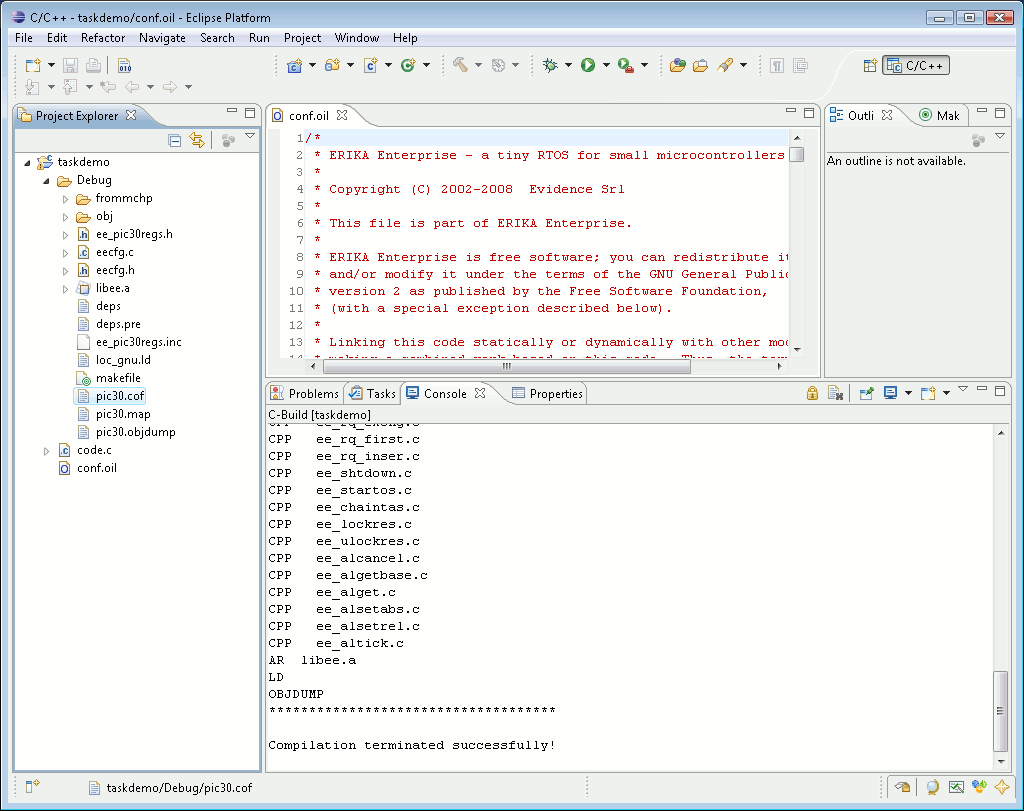
\includegraphics[width=12cm, bb=0 0 1024 811]{images/cof_image.png}
  \end{center}
  \caption{The Eclipse workspace and the \rtd\ plugins for \dspic.}
  \label{fig:eclipse_pic30_workspace}
\end{figure}

Application compilation is also done inside the Eclipse Framework. In
fact, the \rtd\ code generator is able to generate the \ee\
configuration files together with a set of configuration files
(typically, a \file{makefile} plus a set of \file{.c} files) which are
then used to compile the source code.

After that, compilation is started automatically by pressing on the
``Build Project'' menu item inside the ``Project'' menu, which
automatically calls the underlying \file{make} application provided by
the Cygwin environment. As an alternative, the ``Build Project''
command is also available by right clicking on the project name.

The choice of the Cygwin environment has been done to simplify the
building process of an application: in fact, Cygwin provides a set of
traditional Unix tools like \file{make}, \file{awk}, \file{sed}, which
are really useful to implement a command line application building
framework. Moreover, these tools are typically available for free on
Linux platform, easing in this way the porting of the application to a
free development environment such as Linux.


\subsection{Building an application from command line}
The \rtd\ plugins provide three ways to develop an application:
\begin{enumerate}
\item A graphical interface to simplify the development of an
  application, based on Eclipse.
\item A scripting interface based on Apache ANT \cite{ANT}, which is
  the default scripting environment used in the Eclipse Framework.
\item A standalone code generator, that does not use Eclipse.
\end{enumerate}

Using ANT or the standalone version, the developer can automatically
generate from scripts the configuration data and the makefiles which
are then used to compile the application. This removes the need of
opening the graphical environment to compile an application, providing
a way to implement automatic compilation scripts and regression tests.

Please refer to the \rtd\ reference manual for information about ANT
scripting.



\section{Setting up the compiling environment for \dspic}

\ee\ has been designed to be compiled using the GNU gcc toolchain.
The \dspic\ porting of \ee\ in particular can be compiled
using the GNU tools for \dspic\ provided by Microchip. The porting
provides both the \const{binutils} package and the \const{gcc}
package, plus a set of proprietary libraries from Microchip which can
be used to control the various peripherals provided by the \dspic\
microcontrollers.

The following list describes the various packages which contains the
various parts of the compilation toolchain:
\begin{description}
\item[The GNU assembler and binutils.] This package is distributed
  inside the MPLAB IDE from Microchip.
\item[The GNU GCC from Microchip.] The compiler is packaged in a
  separate product, called {\em The Microchip C30 Compiler}, which is
  available as a product under the Microchip website. A free version
  is also available for students and universities. The source code of
  the compiler is also available under the GPL license on the
  Microchip web site.
\item[The GNU GCC recompiled from Microchip sources.] In addition to
  the Microchip C30 Compiler, Evidence also offer a free version of
  the GCC toolchain for \dspic\ compiled from the sources made available
  under the GPL license on the Microchip web site. This version can be
  used to compile \ee\ without additional packages other
  than MPLAB IDE.
  \begin{warning}
    Please note that the free version of the gcc compiler recompiled
    from the Microchip sources is not a {\em full} replacement for the
    Microchip C30 compiler. The Microchip C30 compiler includes many
    features like include files and libraries to control the \dspic\
    peripherals which are not available as open-source.
  \end{warning}
\item[C Libraries.] A set of libraries which can be used to control
  the peripherals implemented on the particular Microchip chip in
  use. These libraries are packaged together with the Microchip C30
  Compiler.
\end{description}

To compile an \ee\ application, the development
environment needs to be configured to correctly recognize the
Microchip C30 compiler and the MPLAB ASM30 assembler programs. For
doing so, please go to the ``Preference'' menu, as shown in Figure
\ref{fig:preferences-menu}, and find the ``RT-Druid/Oil/PIC30
Configurator'' form as depicted in Figure \ref{fig:preferences-pic30}.
The first textbox, labeled \const{Gcc path}, refers to the
installation directory of the Microchip C30 compiler. The second
textbox, labeled \const{Asm path}, refers to the installation
directory of the ASM30 assembler provided with the MPLAB IDE.

Moreover, Figure \ref{fig:preferences-pic30} contains the following
checkboxes:
\begin{description}
\item[Use EE gcc to resolve dependencies] When checked, the C30
  compiler recompiled by Evidence from the Microchip sources will be
  used instead of the installed C30 compiler to compute the
  dependencies of the .C and .S files, and to perform the C
  preprocessing of the .S files. This feature is useful to avoid
  compilation problems when the system has a Student Edition of the
  C30 compiler with an expired license. In that case, the compiler
  puts a message on the standrd output, corrupting the dependencies
  and preprocessing outputs.
\item[Use EE gcc to compile] When checked, the C30 compiler recompiled
  by Evidence from the Microchip sources will be used instead of the
  C30 compiler to compile the .C files. Please note that the original
  Microchip Libraries will be linked also in this case.
\end{description}

\begin{warning}
The install directories specified in the two textboxes of Figure
\ref{fig:preferences-pic30} does {\em not} include the \file{bin}
directory! 

That is, \file{c:\\Programmi\\Microchip\\MPLAB C30} is correct, wheras
\file{c:\\Programmi\\Microchip\\MPLAB C30\\bin} is not.
\end{warning}

\begin{warning}
The install directory of the assembler refers to the assembler
provided with MPLAB IDE and {\em not} the assembler provided with the
C30 compiler. The reason is that the directory is used to call the
assembler and {\em also} to copy the \file{crt0.s} file, which has a
different position in the two assemblers distributions made by
Microchip.
\end{warning}

\begin{warning}
If you are using a Student Editon of the Microchip C30 compiler which
has an {\bf expired license}, please check the ``Use EE gcc to resolve
dependencies'' checkbox in Figure \ref{fig:preferences-pic30}.
\end{warning}

\begin{figure}[htb]
\begin{center}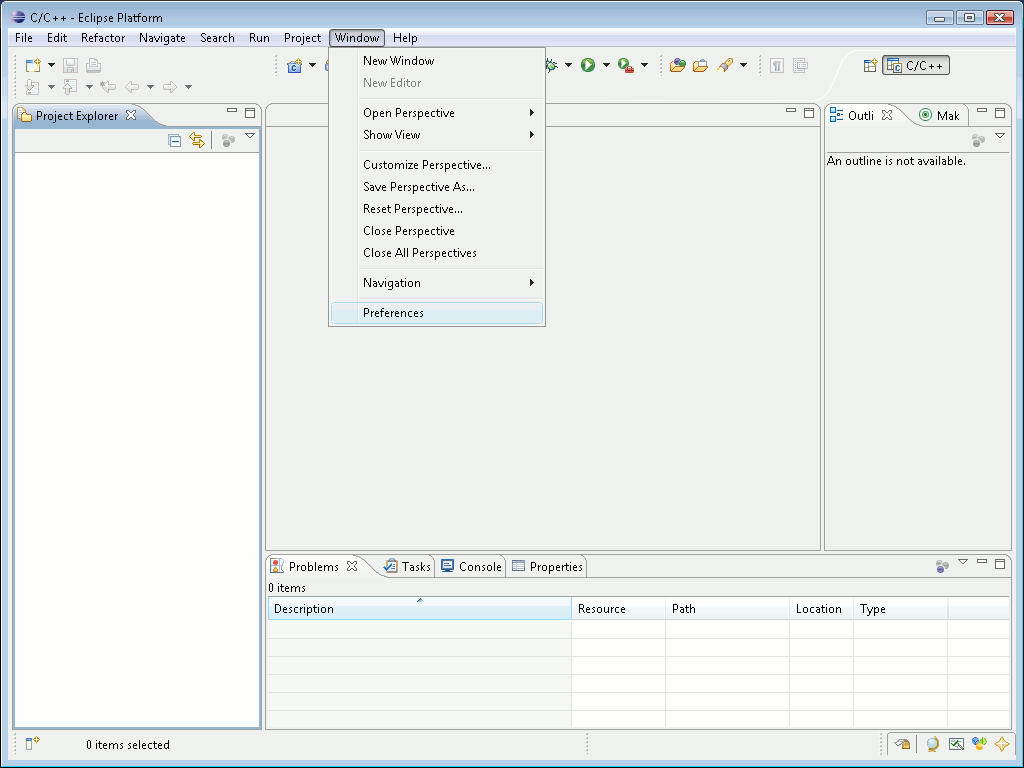
\includegraphics[
  width=8cm, bb=0 0 1024 768]{images/preferences_menu.png}\end{center}
\caption{Go to the ``Preference'' menu.}
\label{fig:preferences-menu}
\end{figure}

\begin{figure}[htb]
\begin{center}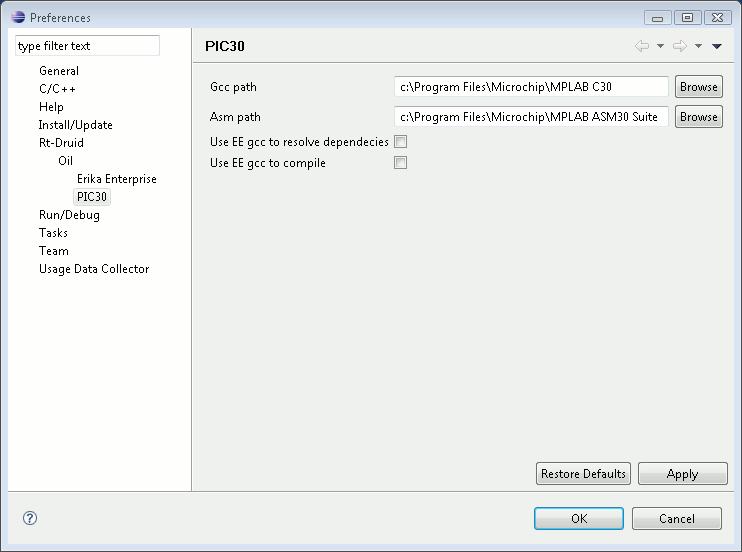
\includegraphics[
  width=8cm, bb=0 0 742 552]{images/preferences_pic30.png}\end{center}
\caption{Select paths for compiler and assembler.}
\label{fig:preferences-pic30}
\end{figure}


\section{Writing software for \dspic\ using \ee}

\begin{note}
Writing an application for \dspic\ using \ee\ is
very simple. Please refer to the \ee Tutorial for the \dspic\
architecture for a step-by-step guide with screenshots on how to
create, compile and debug a \dspic\ application written with \ee.
\end{note}

This section describes the details about the various
configuration options which are available to create and compile an
\ee\ application for a \dspic\ microcontroller.

\begin{note}
For a complete description of all the OIL parameters, please refer to
the \rtd\ reference manual.
\end{note}

\subsection{Avoid the generation of dependency files}
The typical compilation process of an \ee\ application involves the
computation of a dependency file which is used to understand which are
the files which needs to be compiled or updated.

To avoid the computation of these dependencies (useful when you are
sure you basically have to compile everything), you can put the
following line in the OIL file:

\begin{lstlisting}
CPU mySystem {
  OS myOs {
    EE_OPT = "NODEPS";
    ...
  };
  ...
};
\end{lstlisting}

\subsection{Avoid the generation of .src files from C files}
The typical compilation process of an \ee\ application produces
various files which can be used to better analyze the code generated
by the C30 compiler. In particular, from each .C file, a .SRC file is
produced containing the corresponding assembler listing, which is then
compiled by the MPLAB ASM30 compiler to produce the .o.

It is possible to avoid the intermediate step which leads to the
production of the .SRC file. In that case, the compiler will be
responsible of producing the .O file directly from the .C file. This
in general also speeds up the compilation process a little bit.

To obtain that feature, you can put the following lines in the OIL
file.

\begin{lstlisting}
CPU mySystem {
  OS myOs {
    EE_OPT = "NOSRC";
    ...
  };
  ...
};
\end{lstlisting}

\subsection{Printing the commands executed (verbose mode)}

The default compilation process typically prints only a compact output
for each compilation step. That is in general not useful whenever a
file is not compiled properly and the user wants to know the exact
command which is executed in the compilation process.

To obtain a printing of the complete list of commands issued by the
\ee\ makefile, you can add the following line to the OIL file:

\begin{lstlisting}
CPU mySystem {
  OS myOs {
    EE_OPT = "VERBOSE";
    ...
  };
  ...
};
\end{lstlisting}

\subsection{Source files composing an application}
The source files which can be put in an \rtd\ project are composed by
C-language files (with extension \file{.c}) and Assembler files (with
extension \file{.S}). Assembler files are always preprocessed by the C
preprocessor. All the application files which has to be included in
the final application needs to be listed inside the OIL file, as in
the following OIL example:

\begin{lstlisting}
  ...
  CPU_DATA = PIC30 {
    ...
    APP_SRC = "file_1.c";
    APP_SRC = "file_2.c";
  };
  ...
\end{lstlisting}

% /toOl: commented
%\nb{inserire screenshot del configuratore grafico!!}



\subsection{Stack handling}
\ee\ can be configured as monostack or multistack.

In a monostack configuration, only a single stack exists in the
system. No blocking primitives are supported, and all the tasks and
interrupts execute on the same stack. In this case, the one and only
stack starts from the top of the application allocated memory, growing
towards higher addresses. The monostack configuration can {\em not} be
used if the application needs to call RTOS primitives such as
\fn{WaitSem} and \fn{WaitEvent}. Moreover, it cannot be used when \ee\
conformance classes ECC1 and ECC2 are used.

To configure a monostack kernel in the OIL file, the user has to write
the following lines:

\begin{lstlisting}
  ...
  CPU_DATA = PIC30 {
    ...
    MULTI_STACK = FALSE;
  };
  ...
\end{lstlisting}


In a multistack configuration, the kernel support the existence of
different stacks in the same application. Having different stacks
allow the application tasks to use blocking primitives like
\fn{WaitSem} and \fn{WaitEvent}, which basically may block the
execution of the running task. In that case, the calling task must have
a {\em private} stack which is changed upon blocking. The stack will
be selected again when the task will be rescheduled. There are
different stacks available in a multistack configuration:
\begin{itemize}
\item A shared stack (used by all the tasks which have a shared
  stack);
\item An IRQ stack (used by all the ISR Type 2 routines);
\item A set of private stacks (one for each task which has selected a
  private stack).
\end{itemize}

In the \dspic\ architecture, the shared stack works as in the monostack
configuration, that is it is allocated at the end of the application
data section, growing towards higher addresses. The IRQ stack and the
private stacks, instead, are allocated in the application data space
as arrays.

The following example shows an OIL configuration which configures a
multistack kernel without a separate IRQ stack (in this case, IRQ
handlers execute on the stack of the interrupted task):

\begin{lstlisting}
  ...
  CPU_DATA = PIC30 {
    ...
    MULTI_STACK = TRUE {
      IRQ_STACK = FALSE;
    };
  };
  ...
\end{lstlisting}

The following example shows an OIL configuration which configures a
multistack kernel with a separate IRQ stack (in this case, some
registers are saved on the stack of the interrupted task, but the IRQ
handler C function is executed on a separate IRQ stack).

\begin{lstlisting}
  ...
  CPU_DATA = PIC30 {
    ...
    MULTI_STACK = TRUE {
      IRQ_STACK = TRUE {
	SYS_SIZE=64;
      };
    };
  };
  ...
\end{lstlisting}

% /toOl: commented
%\nb{inserire screenshot del configuratore grafico!!}



\subsection{Runtime stack checking exceptions}
When multistack configurations are used, it is very useful to be
informed when a particular stack becomes full. For this reason, the
\dspic\ core allows the user to specify a stack limit over
which an exception should be raised. The stack limit is contained
inside the internal register \const{SPLIM}.

\ee\ is able to automatically handle the \const{SPLIM}
register, setting it at runtime to the top of the current stack when a
multistack configuration.

The \const{SPLIM} feature is by default disabled, because it adds some
(little) overhead at each stack change. To enable it, you must include
the following lines inside the OIL configuration file:

\begin{lstlisting}
  ...
  CPU_DATA = PIC30 {
    ...
    ENABLE_SPLIM = TRUE;
  };
  ...
\end{lstlisting}

% /toOl: commented
%\nb{inserire screenshot del configuratore grafico!!}

Please note that \ee\ does not provide a default handler for the stack
overflow exception generated by the \const{SPLIM} register. The
exception should be specified by the developer as the behavior to
implement is often application dependent.


\subsection{Interrupt handling}
\ee\ for \dspic\ provide support for fast Interrupt Service
Routines (ISR) which do not require any RTOS primitive to be called,
as well as regular ISRs, which can call RTOS primitives (e.g., a timer
interrupt can call \fn{ActivateTask} to activate a periodic task). The
first kind of ISRs are called {\em ISR Type 1}, and always have
hardware interrupt priority greater than the second kind of ISRs which
are called {\em ISR Type 2}.

At the implementation level, \ee\ uses the \dspic\ \fn{DISI} assembler
instruction to implement interrupt disabling. The \fn{DISI}
instruction only disables the first 6 priority levels out of the 7
available in the 16-bit \dspic\ core.

For this reason, ISR Type 2 must always have an interrupt priority
between 1 and 6. ISR Type 1 must always have a priority greater or
equal than ISR Type 2. As a matter of fact, interrupt priority 7 is
reserved for ISR Type 1 only.

ISR names follow the Microchip convention. Basically the ISR names are
listed inside the linker script for the particular target which are
provided together with the ASM30 assembler packaged together with
Microchip MPLAB IDE under the directory
\file{<MPLAB_install_directory>/MPLAB ASM30 Suite/Support/gld}.

To define an ISR Type 1 the developer has to write an interrupt
handler as it is written in typical \dspic\ applications which does not
use \ee. Here is an example of the definition of an ISR Type 1 for the
timer 3 Interrupt of a \const{pic30F2010} device:

\begin{lstlisting}
void __attribute__((__interrupt__)) _T3Interrupt(void)
{
  ...
}
\end{lstlisting}

Writing an ISR 1 in this way implies that:
\begin{itemize}
\item The C function will be attached to the interrupt of the
  peripheral (in the example, timer 3). Every time an interrupt for
  the peripheral arrives, then the C function will be executed.
\item The compiler will generate a proper function prologue and
  epilogue which saves the register used before starting executing the
  statements inside the function. The registers will be saved inside
  the stack of the interrupted task. For that reason, when using a
  multistack configuration, the user should reserve a proper space
  able to contain all the nested ISR Type 1 {\em for each} stack in
  the system.
\end{itemize}

To define an ISR Type 2 the developer has to write a C function in the
following way:

\begin{lstlisting}
#include "cpu/pic30/inc/ee_irqstub.h"
...
ISR2(_T3Interrupt)
{
  ...
}
\end{lstlisting}

Writing an ISR 2 in this way implies that:
\begin{itemize}
\item An assembler stub will generated for the ISR. The ISR stub will
  have the name of the ISR (in the example, \fn{_T3Interrupt}). The
  assembler stub will call a C function named \fn{ISR2\_functionname}
  which content is specified as the content of the function (in the
  example, the function is called \fn{ISR2\_\_T3Interrupt}). The
  assembler function will be attached to the interrupt of the
  peripheral (in the example, timer 3). Every time an interrupt for
  the peripheral arrives, the assembler stub will execute,

  which in turns calls the internal C function whose body has been
  specified by the developer.
\item The assembler stub saves {\em all} the CPU registers on the
  current stack. After that, if a multistack configuration with
  private IRQ stack has been selected, the stack is changed to a
  private IRQ stack. Otherwise, the ISR will execute on the stack of
  the running task, as in the ISR1 case.  At the end of the stub, the
  \ee\ end IRQ function will be executed to choose which is the next
  task to run.
\end{itemize}




\subsection{Configuring the usage of Microchip ICD2}
\dspic\ devices can be debugged using the Microchip product
called Microchip ICD2, which is basically an In-Circuit debugger which
directly connects to the microcontroller core. When connected, the
ICD2 requires the usage of a set of memory locations, which must be
left free by the application.

For this reason, when compiling an application which will be debugged
using the Microchip ICD2, the user has to specify the following line
inside the OIL file:

\begin{lstlisting}
  ...
  CPU_DATA = PIC30 {
    ...
    ICD2 = TRUE;
  };
  ...
\end{lstlisting}

% /toOl: commented
%\nb{inserire screenshot del configuratore grafico!!}




\subsection{Configuring a particular \dspic\ microcontroller}

Microchip produces various versions of the Microchip microcontrollers,
each one with different peripherals and memory sizes. To support the
heterogeneity of these devices, Microchip offers, through the C30
Compiler toolchain, a set of files which can be used to configure the
compiling process.

In particular, for each device, there are four files:
\begin{itemize}
\item A linker script, available under the directory
  \file{Support/gld} of the Microchip ASM30 Assembler, which contains the
  linking information such as the memory sizes, and the available
  interrupt handlers;
\item An Assembler include file, available under the directory
  \file{Support/inc} of the Microchip ASM30 Assembler, which contains the
  declaration of the device's register addresses to be used inside
  assembler programs;
\item A C include file, available under the directory \file{support/h}
  of the Microchip C30 Compiler, which contains the declaration of the
  device's addresses to be used inside C programs;
\item A library, available under the directory \file{lib} of the
  Microchip C30 compiler, which contains a set of libraries for the
  usage of the microcontroller peripherals.
\end{itemize}

Every \ee\ application which has to be compiled together with the
Microchip C30 compiler needs the specification of these four files. To
set which files have to be used for the particular device, the user
can specify the following lines inside the OIL file.

If the device number is known, and the files to be used are the
default files provided by Microchip, then the developer can directly
specify the device name in the OIL file, as in the following example:

\begin{lstlisting}
  ...
  MCU_DATA = PIC30 {
    MODEL = PIC33FJ256GP710;
  };
  ...
\end{lstlisting}

Currently, \ee\ supports the following values for the \const{MODEL}
attribute:
\begin{itemize}
\item PIC24 devices: \newline
  \const{PIC24FJ128GA006}, \const{PIC24FJ128GA008},\newline
  \const{PIC24FJ128GA010}, \const{PIC24FJ32GA002},\newline
  \const{PIC24FJ32GA004}, \const{PIC24FJ64GA002},\newline
  \const{PIC24FJ64GA004}, \const{PIC24FJ64GA006},\newline
  \const{PIC24FJ64GA008}, \const{PIC24FJ64GA010},\newline
  \const{PIC24FJ96GA006}, \const{PIC24FJ96GA008},\newline
  \const{PIC24FJ96GA010}, \const{PIC24HJ128GP206},\newline
  \const{PIC24HJ128GP210}, \const{PIC24HJ128GP306},\newline
  \const{PIC24HJ128GP310}, \const{PIC24HJ128GP506},\newline
  \const{PIC24HJ128GP510}, \const{PIC24HJ256GP206},\newline
  \const{PIC24HJ256GP210}, \const{PIC24HJ256GP610},\newline
  \const{PIC24HJ64GP206}, \const{PIC24HJ64GP210},\newline
  \const{PIC24HJ64GP506}, \const{PIC24HJ64GP510}.
\item PIC30 devices: \newline
  \const{PIC30F1010}, \const{PIC30F2010}, \newline
  \const{PIC30F2011}, \const{PIC30F2012}, \newline
  \const{PIC30F2020}, \const{PIC30F2021}, \newline
  \const{PIC30F2022}, \const{PIC30F2023}, \newline
  \const{PIC30F3010}, \const{PIC30F3011}, \newline
  \const{PIC30F3012}, \const{PIC30F3013}, \newline
  \const{PIC30F3014}, \const{PIC30F4011}, \newline
  \const{PIC30F4012}, \const{PIC30F4013}, \newline
  \const{PIC30F5011}, \const{PIC30F5013}, \newline
  \const{PIC30F5015}, \const{PIC30F5016}, \newline
  \const{PIC30F6010}, \const{PIC30F6010A}, \newline
  \const{PIC30F6011}, \const{PIC30F6011A}, \newline
  \const{PIC30F6012}, \const{PIC30F6012A}, \newline
  \const{PIC30F6013}, \const{PIC30F6013A}, \newline
  \const{PIC30F6014}, \const{PIC30F6014A}, \newline
  \const{PIC30F6015}.
\item PIC33 devices: \newline
  \const{PIC33FJ128GP206}, \const{PIC33FJ128GP306},\newline
  \const{PIC33FJ128GP310}, \const{PIC33FJ128GP706},\newline
  \const{PIC33FJ128GP708}, \const{PIC33FJ128GP710},\newline
  \const{PIC33FJ128MC506}, \const{PIC33FJ128MC510},\newline
  \const{PIC33FJ128MC706}, \const{PIC33FJ128MC708},\newline
  \const{PIC33FJ128MC710}, \const{PIC33FJ256GP506},\newline
  \const{PIC33FJ256GP510}, \const{PIC33FJ256GP710},\newline
  \const{PIC33FJ256MC510}, \const{PIC33FJ256MC710},\newline
  \const{PIC33FJ64GP206}, \const{PIC33FJ64GP306},\newline
  \const{PIC33FJ64GP310}, \const{PIC33FJ64GP706},\newline
  \const{PIC33FJ64GP708}, \const{PIC33FJ64GP710},\newline
  \const{PIC33FJ64MC506}, \const{PIC33FJ64MC508},\newline
  \const{PIC33FJ64MC510}, \const{PIC33FJ64MC706},\newline
  \const{PIC33FJ64MC710}.
\end{itemize}

Please note that we did not have the possibility to directly test {\em
all} the possible devices produced by Microchip. In general this is
not a problem, because the various devices are directly mapped to
appropriate compiler flags. The following is the list of devices we
tested directly: \const{PIC30F2010}, \const{PIC30F6014A},
\const{PIC33FJ256GP710}, \const{PIC24FJ128GA010}, which basically are
the devices mounted on the Microchip Evaluation boards supported by
\ee.


If the device is not supported by the particular version of \rtd\, or
if the developer needs to use a custom file, then the four files can
be specified separately as in the following example:

\begin{lstlisting}
  ...
  MCU_DATA = PIC30 {
    MODEL = CUSTOM {
      MODEL = "33FJ256GP710";
      LINKERSCRIPT = "p33FJ256GP710.gld";
      DEV_LIB = "libp33FJ256GP710-elf.a";
      INCLUDE_C = "p33FJ256GP710.h";
      INCLUDE_S = "p33FJ256GP710.inc";  
    };
  };
  ...
\end{lstlisting}

As a result of this specification, the correct include files,
libraries and linker scripts will be used when compiling an \ee\
application.

% /toOl: commented
%\nb{Includere uno screenshot!}


% /toOl: commented
%\section{Integrating \ee\ with Microchip and third party libraries}
%
%\nb{Nino: cosa si pu� scrivere sull'uso dei device drivers microchip e 
%delle librerie fornite con il compilatore C30?
%}


\section{Configuring the EDF scheduler}

When configuring the EDF kernel for an \ee\ application, the user has
the possibility to specify the tick length in the OIL file to allow
the specification of a relative deadline using a temporal value.

In particular, the user can specify a tick value as follows:

\begin{lstlisting}
  KERNEL_TYPE = EDF {TICK_TIME = "25ns";};
\end{lstlisting}

and then specify a relative deadline using a timing value as follows:

\begin{lstlisting}
  TASK myTask1 {
    REL_DEADLINE = "10ms";
  };
\end{lstlisting}

The \rtd\ code generator will handle the the conversion between the
relative deadline value in the corresponding timing value
automatically.

The important thing in this process is to correctly specify the
\const{TICK_TIME}. In general, that value depends on the timing
reference which is made available by the \dspic. The current timing
reference implemented in the EDF kernel is based on the value of a 32
bit timer.

Having a 32 bit timing reference helps implementing a long lifetime
for the circular timer, allowing the support of relatively long
relative deadlines.

The 32 bit timer is obtained by concatenating the two 16 bit timers
\const{TMR8} and \const{TMR9} available on the \dspic. The clock used
for the timers is the system clock, with a tick time equal to
$\frac{1}{F_{cy}}$, where $F_{cy} = \frac{F_{osc}}{2}$. $F_{osc}$, the
frequency of the oscillator, depends on its configuration which is
typically done in the application by using appropriate macros shown
below.

The following paragraphs describe two typical oscillator values which
can be used, and the correspondent parameters which has to be put in
the OIL file. The same settings are available in two template
applications distributed with \ee\, which work on the \flex\ boards
featuring a \dspic\ model \const{PIC33FJ256MC710}.

Finally, always remember that the \reffun{EE_time_init} function has
to be called inside the \fn{main} function before using any primitive
of the EDF kernel.


\subsection{Primary oscillator without PLL}

In this configuration, a primary oscillator at 4 MHz is used without
any moltiplication. In this case, the tick duration is 500 ns, and the
\dspic\ is running at 2 MIPS.

To configure the system in this way, the C language has to contain the
following compiler directive:

\begin{lstlisting}
  _FOSCSEL(FNOSC_PRI);
\end{lstlisting}

The OIL file will contain the following line:

\begin{lstlisting}
  KERNEL_TYPE = EDF {TICK_TIME = "500ns";};
\end{lstlisting}

The maximum relative deadline which can be expressed in the OIL file
is $500 ns * 2^{31}$, which is slightly more than 1073 secs.

A template application which initializes an EDF periodic task for this
case is available under the \rtd\ templates.

\subsection{Primary oscillator with PLL}

In this configuration, the \dspic\ is configured to provide its
maximum computational power. To do that, the internal PLL is used to
push the internal frequency $F_{osc}$ to 80 MHz. As a consequence,
$F_{cy}$ become 40 MHz, which is the nominal maximum computational
power of 40 MIPS declared by Microchip. In this case, the tick
duration is 25 ns.

To configure the system in this way, the C language has to contain the
following compiler directive:

\begin{lstlisting}
  _FOSCSEL(FNOSC_PRIPLL);
\end{lstlisting}

Moreover, at the beginning of the \fn{main} function, the PLL
multiplier registers needs to be set with the following code:

\begin{lstlisting}
  /* Clock setup for 40MIPS */
  CLKDIVbits.DOZEN   = 0;
  CLKDIVbits.PLLPRE  = 0;
  CLKDIVbits.PLLPOST = 0;
  PLLFBDbits.PLLDIV  = 78;
  
  /* Wait for PLL to lock */
  while(OSCCONbits.LOCK!=1);
\end{lstlisting}

Finally, the OIL file will contain the following line:

\begin{lstlisting}
  KERNEL_TYPE = EDF {TICK_TIME = "25ns";};
\end{lstlisting}

The maximum relative deadline which can be expressed in the OIL file
is $25 ns * 2^{31}$, which is slightly more than 53 secs.


\begin{function_nopb2}{EE\_time\_init}{EE_time_init}
  \synopsis{void EE_time_init(void);}
  
  \begin{fundescription}
    The function programs \const{TMR8} and \const{TMR9} as a 32 bit
    timer which is then used by the EDF Kernel to take the timing
    reference.

    The function {\em must} be called before calling any \ee\
    primitive.
  \end{fundescription}
  
%  \begin{funparameters}
%    \fpar{none}{None in this function.}
%  \end{funparameters}
  
%  \begin{funreturn}
%    \fret{void}{The function does not return a value.}
%  \end{funreturn}
  
%  \begin{funconformance}
%  \end{funconformance}
\end{function_nopb2}

